% NOTES
% the tilde ~ (alt-n) creates a non-breaking space, which is needed in the tables to prevent LaTeX from removing spaces (actually show 16 character wide lcd-figures)
% ~ \newline % Benötigt, damit Text nicht direkt neben der Paragraphen-Überschrift beginnt
% dashes: hyphen -, en-dash --, em-dash ---, minus-sign $-$


% Präambel
\documentclass[12pt, a4paper, german]{article}
%\usepackage[a4paper, total={6in, 8in}]{geometry}
\usepackage[T1]{fontenc}
\usepackage[utf8]{inputenc}
\usepackage{babel}
\usepackage[all]{xy}
\usepackage{courier}
\usepackage{graphicx}

\title{Dokumentation des Projekts "Sequenzer mit Tonerzeugung" im Modul Programmiertechnik}
\author{Daniel Erich Raab und Justus Konstantin Schmidt}
\begin{document}

% LC-Display Abbildungs-Makros
% leeres Display:
 % ~ & ~ & ~ & ~ & ~ & ~ & ~ & ~ & ~ & ~ & ~ & ~ & ~ & ~ & ~ & ~ \\
 % ~ & ~ & ~ & ~ & ~ & ~ & ~ & ~ & ~ & ~ & ~ & ~ & ~ & ~ & ~ & ~ \\
\def\startlcdtable{
	\begin{figure}[h]
	\ttfamily
	\centering
	\setlength{\tabcolsep}{2pt} % makes the columns narrower (standard is 5pt)
	\begin{tabular}{|cccccccccccccccc|}
	\hline
}
\def\endlcdtable#1#2{
	\hline
	\end{tabular}
	\normalfont
	\caption{#1}
	\label{#2}
	\end{figure}
}

% Makro für Auszüge des Displays im Text
\newcommand{\lcdtext}[1] {\texttt{\framebox[1.1\width]{#1}}}

% Makro für Funktionennamen, bzw. allgemein Namen aus dem source code
\newcommand{\source}[1] {\texttt{#1}}

% Makro für xy-Zeichnungen
\newcommand{\xydiagram}[3]{
	\begin{figure}[h]
	\centering
	\[
	\begin{xy}
	\xymatrix {
		#1
	}
	\end{xy}
	\]
	\caption{#2}
	\label{#3}
	\end{figure}
}

% ANMERKUNGEN
% Unterstrich kann nicht direkt eingegeben werden, sondern es muss ein \ vorangestellt werden
% für Funktionsnamen bzw. allgemein code verwende bitte: \source{NAME}
% Für Unterüberschriften, die nicht im Inhaltsverzeichnis erscheinen: \paragraph{TITEL} ~ \newline

% Titelseite und Inhaltsverzeichnis
\maketitle
\tableofcontents

% Die Texte sind diesen seperaten Dateien
\section{Vorwort}
Dies ist die technische Dokumentation des Projekts im Modul Programmiertechnik von Daniel Raab und Konstantin Schmidt. Es wird der Aufbau der Software beschrieben und dargestellt, sowie die einzelnen Teilmodule. Das Projekt wurde für das \emph{MSP Education Board 3.0} der HTWK Leipzig entworfen und implementiert. Der Quellcode wurde in C mithilfe des \emph{Code Composer Studio 6} geschrieben.
\section{Struktur}
\subsection{Grundstruktur}
Das Programm besitzt keinen sequentiellen Ablauf, da ein auf interrupts(engl. Unterbrechungen) basierender Ansatz gewählt wurde, um alle Funktionen gut implementieren zu können.
\begin{figure}[h]
    \centering
    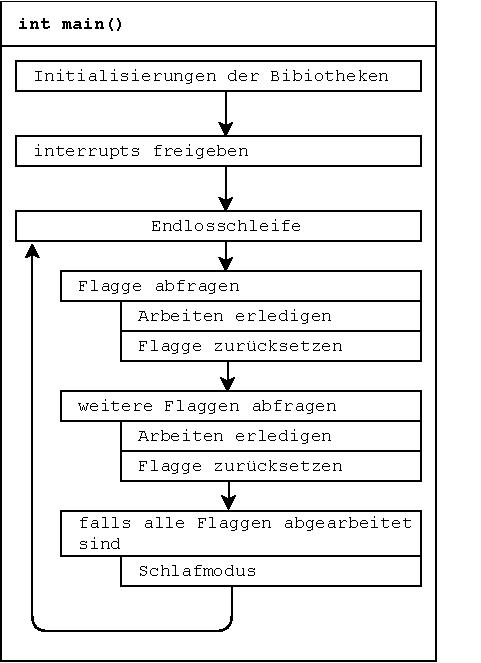
\includegraphics{main_diagram.pdf}
    \caption{Der Grundablauf schematisch dargestellt}
    \label{img:grundablauf}
\end{figure}
\newline
Der Grundablauf ist in Abbildung \ref{img:grundablauf} zusehen. Es wird zuerst der Mikrorechner und alle benötigten Systeme initialisiert und dann in den interrupt-gesteuerten Betrieb übergegangen. Der Prozessor wird also in den Schlaf- bzw. Low-Power-Modus versetzt und reagiert ab sofort nur noch auf auftretende interrupts. Die aufgerufene interrupt service routine (ISR) soll möglichst schnell abgearbeitet werden, also wird meist lediglich das interrupt ausgewertet und dann eine entsprechende Flagge gesetzt. Dann wird der Schlafmodus verlassen und die ISR beendet. Durch das Verlassen des Schlafmodus werden nun in der main()-Funktion die nächsten Befehle ausgeführt. Hier werden nun die Flaggen abgefragt und die entsprechenden Arbeiten erledigt. Sobald alle Flaggen abgefragt und abgearbeitet sind, wird der Prozessor wieder in den Schlafmodus versetzt. Diese Abarbeitung in der main()-Funktion hat den großen Vorteil, dass lang andauernde Arbeiten, wie z.B. Ansteuerung des Displays mit Wartezeiten, durch interrupts unterbrochen werden können, ohne das erst auf die lange andauernden Anweisungen gewartet werden muss. Diese Blockierung der schnell abzuarbeitenden ISRs passiert, wenn alle Aufgaben in ISRs passieren und nicht in der main()-Funktion. Zeitkritische Aufgaben z.B. Tastendrücke oder Töne könnten nicht richtig oder zeitnah ausgelesen bzw. ausgegeben werden. Eine Ausnahme dieser Regel betrifft die \source{play\_tone}-Funktion der Tonbibliothek, siehe .%TODO: ref

\subsection{Modulstruktur}
Die Programmierung des Mikrorechners erfolgte in Teilmodulen, die sich den verschiedenen Teilbereichen des Projekts widmen. Diese Teilmodule des Projekts wurden erst für sich entwickelt und sobald ein passabler Grad der Implementierung erreicht wurde in das Gesamtprojekt eingebunden und im Verbund getestet. Das Projekt wurde in folgende Module zerlegt:
\begin{itemize}
    \item Sequenz-Datenstrukturen (\textsl{sequence.h})
	\item Display-Ansteurung (\textsl{lcd.h})
	\item Eingaben, also Taster und Drehgeber (\textsl{input.h})
	\item Tonerzeugung (\textsl{tone.h})
	\item LED-Matrix (\textsl{led\_matrix.h})
\end{itemize}
Die Steuerung des Programms passiert in der \textsl{main.c} über die Funktionen, die auf die Eingaben des Benutzers reagieren. Dort werden alle Bibliotheken und Module eingebunden und zum Projekt vereinigt.

\section{Module}
Hier werden die Module genauer in ihrem Aufbau und ihrer Struktur beschrieben. Die Modulnamen für die tatsächlichen Dateien sind in Klammern angegeben und umfassen die entsprechende *.h und *.c Dateien.

\subsection{\source{main.c}}
Die \source{main.c}-Datei ist der Einstiegspunkt des Programms und enthält die Funktion \source{int main()}. Es werden alle unserer Bibliotheken inkludiert, und diese werden gleich zu Beginn durch ihre Initialisierungsfunktionen initialisiert werden können. Danach werden die interrupts freigegeben und das Programm startet die Hauptschleife und damit den interrupt-basierten Ablauf, wie im Abschnitt Grundstruktur und in der Abbildung \ref{img:grundablauf} erläutert.
\newline


Es werden außer den ISRs noch ähnliche Funktionen definiert, die durch Bibliotheken für bestimmte Ereignisse aufgerufen werden. Dies sind \source{void new\_minute()}, das von der Uhrzeit-Bibliothek aufgerufen wird, sobald eine neue Minute angebrochen ist und die Funktion \source{void alarm\_ring()}, die signalisiert, dass ein Alarm ausgelöst worden ist und nun klingeln soll. Diese Funktionen wurden in die \source{main.c} Datei verlegt, da diese Ereignisse Veränderungen in mehreren Bibliotheken auslösen: \source{void new\_minute()} bedeutet, dass die Alarme überprüft werden müssen und die LED-Matrix aktualisiert werden muss;
\source{void alarm\_ring()} bedeutet, dass das Menü in den Alarm-Modus übergehen muss und die Melodie des entsprechenden Alarms gestartet wird.


\subsection{Hauptprogramm (\emph{main})}
Die \source{main.c}-Datei ist der Einstiegspunkt des Programms und enthält die Funktion \source{int main()}. Es werden alle unserer Bibliotheken inkludiert und die Funktionen deklariert, die für die Bedienung der Ereignisse aus den Interrupts zuständig sind. In der Variable \source{mode} wird gespeichert, in welchem der beiden möglichen Modi sich der Sequenzer gerade befindet. \par \noindent 
\source{outdated\_display} ist eine Flagge, die signalisiert, ob das LCD aktualisiert werden muss. Sie wird hier am Ende jeder Funktion gesetzt, weil jede Funktion Einfluss auf die Displayausgabe hat.

\subsubsection{\source{int main()}} % (fold)
\label{ssub:int main}
Gleich zu Beginn werden die einzelnen Systeme initialisiert. Dann werden die Startwerte der Variablen zugewiesen. Dazu gehört auch die Startmelodie, für die jedem der 16 Schritte eine Tonhöhe und eine Tonlänge zugewiesen werden muss. Nachdem LCD und LED-Matrix gestartet wurden, werden die interrupts freigegeben und es startet die Hauptschleife und damit der interrupt-basierte Ablauf, wie im \emph{Abschnitt \ref{sub:grundstruktur} Grundstruktur} und in der Abbildung \ref{img:grundablauf} erläutert.
% subsubsection int main (end)

\subsubsection{\source{void button\_SW1\_pressed()}} % (fold)
\label{ssub:void_button_sw1_pressed}
Wenn der Taster \textbf{SW1} gedrückt wird, wird der Modus gewechselt. Falls vom Bearbeitungsmodus in den Abspielmodus gewechselt wird, wird die Tonerzeugung gestartet und \source{current\_step} auf \source{0} gesetzt, damit die Sequenz vom Anfang an abgespielt wird. \source{update\_tempo(tempo)} wird in \emph{Abschnitt \ref{sub:ton}} erklärt. Die LED-Matrix wird auch aktualisiert.
% subsubsection void_button_sw1_pressed (end)

\subsubsection{\source{void button\_SW2\_pressed()}} % (fold)
\label{ssub:void_button_sw2_pressed}
Mit Taster \textbf{SW2} wird im Bearbeitungsmodus die Tonlänge eingestellt. Sie wird mit jedem Tastendruck erhöht.

\noindent Wenn \source{sequence[current\_step].tone\_length = full} erreicht ist, wird die Tonlänge beim nächsten Tastendruck wieder auf \source{pause} gesetzt.
% subsubsection void_button_sw2_pressed (end)

\subsubsection{\source{void button\_SW3\&4\_pressed()}} % (fold)
\label{ssub:void_button_sw3_pressed}
Taster \textbf{SW3} und \textbf{SW4} verringern und erhöhen das aktuelle Tempo. Wenn die Unter- oder Obergrenze erreicht ist, bewirkt ein weiterer Tastendruck keine Veränderung.
% subsubsection void_button_sw3_pressed (end)

\subsubsection{\source{void encoder\_left\&right()}} % (fold)
\label{ssub:void_encoder_left&right}
Mit dem \textbf{Encoder} wird im Bearbeitungsmodus die Tonhöhe des zu bearbeitenden Schritts eingestellt. Eine Drehung nach links bewirkt eine eine Verringerung der Tonhöhe und eine Drehung nach rechts ein Erhöhung. Wiederum wird der Wert nur verändert, wenn weder Ober- noch Untergrenze erreicht ist.
% subsubsection encoder_left&right (end)

\subsubsection{\source{void potentionmeter\_turned()}} % (fold)
\label{ssub:void_potentionmeter_turned}
Im Bearbeitungsmodus kann mit dem \textbf{Potentiometer} der zu bearbeitende Schritt ausgewählt werden. Dazu wird \source{pot\_value} der aktuellen Schrittnummer \source{current\_step} zugewiesen. Die LED-Matrix wird aktualisiert und die aktuelle Tonhöhe des Schritts wird kurz angespielt.
% subsubsection potentionmeter_turned (end)

\subsubsection{\source{void play\_next\_step()}} % (fold)
\label{ssub:void_play_next_step}
Diese Funktion ist dafür verantwortlich, dass die Sequenz im Abspielmodus kontinuiertlich abgespielt wird. Abhängig von der Tonlänge wird ein Ton mit der Tonhöhe des aktuellen Schritts abgespielt. Die übergebene Tonlänge wird in Hundertstelsekunden übergeben. Da diese abgängig vom Tempo ist, muss sie hier berechnet werden. Der Faktor ergibt sich daraus, dass das Tempo in BPM (engl. beats per minute; \emph{Schläge pro Minute}) angegeben ist. Ein Ton mit der Länge \source{full} dauert also \(\frac{1}{\source{tempo}}*60\) Sekunden. Wenn man das mit 100 multipliziert, kommt man auf das Ergebnis in Hundertstelsekunden.
\[
Tonl\ddot{a}nge~\source{full}~in~Hunderstelsekunden=\frac{1}{\source{tempo}}*60*100=\frac{6000}{\source{tempo}}
\]
Die anderen Tonlängen sind lediglich mit 0.25, 0.5 und 0.75 multipliziert.\newline

Die LED-Matric wird wieder aktualisiert und die Schrittnummer wird inkrementiert, wenn der letzte Schritt noch nicht erreicht ist. Falls doch, wird \source{current\_step} wieder nullgesetzt, sodass die Sequenz wieder von vorne beginnt.
% subsubsection void_play_next_step (end)

\subsubsection{\source{void update\_display()}} % (fold)
\label{ssub:void_update_display}
Immer, wenn die Flagge \source{outdated\_display} beim Durchlaufen der Schleife in \source{int main()} aktiviert ist, wird diese Funktion aufgerufen. Hier werden alle Funktionen aufgerufen, die für das Beschreiben des LC-Displays zuständig sind.
% subsubsection void_update_display (end)
% ANMERKUNGEN
% Unterstrich kann nicht direkt eingegeben werden, sondern es muss ein \ vorangestellt werden
% für Funktionsnamen bzw. allgemein code verwende bitte: \source{NAME}
% Für Unterüberschriften, die nicht im Inhaltsverzeichnis erscheinen: \paragraph{TITEL} ~ \newline

\subsection{Display (\emph{lcd})}
Die Display Bibliothek steuert das LC-Display und stellt verschiedene Methoden zur Beschreibung dessen zur Verfügung.
Außerdem werden besondere Zeichen, hier eine Glocke, in das Display einprogrammiert und gespeichert. Das Display besitzt einen Cursor, der bestimmt wo neue Zeichen geschrieben werden.
\newline
Alle Funktionen des Display benötigen (relativ) viel Zeit, um mit dem Display-Controller zu kommunizieren und sollten demnach nicht in ISRs benutzt werden.
\subsubsection{\source{void lcd\_init()}}
Das LC-Display wird gestartet und initialisiert über die Funktion \source{void lcd\_init()}. Es wird dann die Initialisierungssequenz für das Display gesendet und es für die weitere Verwendung konfiguriert. Es wird das Display geleert und sowohl der Cursor als auch Blinken ausgeschaltet.
\subsubsection{\source{void lcd\_clear()}}
Eine Funktion, die alles Angezeigte vom Display löscht und den Cursor zurück in die obere, linke Ecke (0, 0) setzt.
\subsubsection{Schreibfunktionen}
Als grundlegenden Schreibfunktionen, um das Display zu verwenden, sind
\begin{itemize}
    \item \source{void lcd\_write(unsigned char character)},
    \item \source{void lcd\_write\_string(unsigned char string[])} und
    \item \source{void lcd\_write\_int(unsigned int number, int digits)}
\end{itemize}
für die verschiedenen wichtigen Datentypen implementiert. Es können einzelne Zeichen (\source{unsigned character}) gesendet werden, sowie ganze strings, also Felder von Zeichen, die jedoch mit dem terminierendem Zeichen \source{0x0} oder \source{'\textbackslash0'} abgeschlossen werden müssen. Dies passiert automatisch, wenn ein string mit doppelten Anführungszeichen angegeben wird. Um Zahlen (\source{int}) anzuzeigen muss noch ein zweites Argument übergeben werden, das die Anzahl der Stellen bestimmt. Falls die Zahl weniger Stellen besitzt, wird der Rest mit Nullen aufgefüllt, also wird beispielsweise bei der Zahl 45 und drei Stellen \lcdtext{045} angezeigt.
\newline
All diese Funktionen schreiben immer ab der aktuellen Position des Cursors und der Cursor ist nach dem Schreiben beim nachfolgenden Zeichen des letzten neu auf das Display geschriebenen Zeichens.
\subsubsection{\source{void lcd\_set\_cursor(unsigned char x, unsigned char y)}}
Der Cursor kann mithilfe der Funktion \source{void lcd\_set\_cursor(unsigned char x, unsigned char y)} an eine beliebige Stelle im Display gesetzt werden. \source{x} steht für die Position innerhalb der Zeile (beginnend mit 0, also maximal 15) und \source{y} für eine der beiden Zeilen (0 oder 1).
\subsubsection{Zeit und Datum}
Es sind außerdem für dieses Projekt spezifische Funktionen implementiert, um eine Uhrzeit mit oder ohne Sekunden anzuzeigen (\source{void lcd\_write\_time(Time time, bool seconds)}), ein Datum mit oder ohne Wochentag anzuzeigen (\source{void lcd\_write\_date(Date date, bool weekdays)}) und das spezielle Zeichen Glocke auf das Display zu schreiben.

\subsection{Eingabe (\emph{input})}
In der Eingabe-Bibliothek werden die Taster sowie der Encoder ausgelesen und dem Rest des Programms in Form von Flaggen zur Auswertung zur Verfügung gestellt. Es werden die interrupts an Port 2 empfangen und ausgelesen, die jeweilige Flagge gesetzt und der Low-Power-Modus beendet, damit die Flaggen sofort ausgelesen und darauf reagiert werden kann.
\subsubsection{\source{void button\_init()}}
Die Funktion initialisiert den Port 2 so, dass die interrupts ausgelöst und damit auf die Eingaben reagiert werden kann.
\subsubsection{Flaggen}
Es gibt für jeden Taster eine Flagge (\source{bool button\_SW4} bis \source{bool button\_SW1} entsprechend der Tasternummer) und zwei für die beiden Drehrichtungen des Encoders (\source{bool encoder\_l} sowie \source{bool encoder\_r}).
\subsubsection{\source{\_\_interrupt void P2\_ISR()}}
Die interrupt service routine für Port 2, die aufgerufen wird, sobald ein Taster oder der Encoder betätigt werden. Dort wird überprüft, ob der Encoder und wenn ja, in welche Richtung er gedreht wurde. Da die Taster prellen, dürfen die Tasterdrücke nicht sofort ausgewertet werden, da ansonsten bei jedem Tastendruck fälschlicherweise viele Tastendrücke erkannt werden würden. Deswegen wird über die Wartefunktion \source{void debounce\_delay()} eine passende Wartezeit vor der Auswertung realisiert. Je nachdem welche Taster oder Encoder-Richtung erkannt wurde, wird die entsprechende Flagge gesetzt und der Prozessor aus dem Schlafmodus aufgeweckt, um in der \source{main()}-Funktion darauf zu reagieren.


\end{document}
